\appendixpage
\section{Representative constructions}
\label{app:cases}
\newcommand{\CaseCapRatio}{0.970}
\newcommand{\CaseShannonReference}{1,941,100,559,147}
\newcommand{\CaseShannonRatio}{0.713}
\newcommand{\CaseShannonGain}{38.4}

\subsection{Cap sets: a small ingredient at twice the dimension}
\label{case:capset}
\textbf{Model:} GPT-6 Astra, high effort, tool-free. \textbf{Instance:} $d=12$, problem-size experiment.

\begin{taskbox}[title=Task]
Construct a subset of $\mathbb F_3^{12}$ with no three distinct points summing to zero. The objective is the number of points. The published frontier contains 12,928 points.
\end{taskbox}

\begin{center}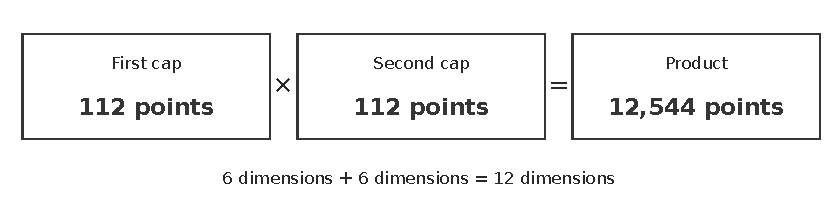
\includegraphics[width=\linewidth]{figs/appendix/case_capset.pdf}\end{center}

\begin{constructionbox}[title=Construction and verification]
The answer takes the Cartesian product of two copies of a 112-point cap $C\subseteq\mathbb F_3^6$:
\[
S=C\times C,\qquad |S|=112^2=12544.
\]
Each finite factor is checked for forbidden triples. In characteristic three, a zero-sum triple in a cap has all three entries equal: three distinct entries are forbidden, and two equal entries force the third to be equal. Applying this fact in each factor shows that any zero-sum triple in $C\times C$ consists of one repeated point.

Both answers at this problem size use this product. The construction makes the dependence on dimension explicit: repeating a factor adds dimensions and multiplies cardinalities.
\end{constructionbox}

\begin{resultbox}[title=Measured quality]
\begin{tabularx}{\linewidth}{@{}XXX@{}}
Model construction & Published frontier & Relative quality \\
\textbf{12,544 points} & 12,928 points & $12544/12928=\mathbf{\CaseCapRatio}$
\end{tabularx}
\end{resultbox}

The product describes a large, valid cap set close to the published frontier using only its smaller factors. The size--quality curves in Appendix~\ref{app:ladder_results} compare how this construction and graph constructions behave as their parameters grow.

\appendixpage
\subsection{Shannon codes: better factors produce a larger code}
\label{case:shannon}
\textbf{Model:} Qwen3.8-27B, high effort, tool-free. \textbf{Instance:} length 24 over seven symbols ($C_7^{24}$).

\begin{taskbox}[title=Task]
Construct codewords of length 24 over $\mathbb Z_7$. Every pair must differ by cyclic distance at least two in some coordinate. The objective is the number of codewords.
\end{taskbox}

\begin{center}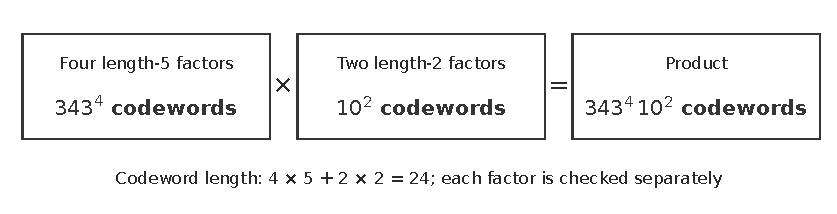
\includegraphics[width=\linewidth]{figs/appendix/case_shannon.pdf}\end{center}

\begin{constructionbox}[title=Construction and verification]
The submitted factors contain 343 words of length five and ten words of length two. Their multiplicities are four and two:
\[
4\cdot5+2\cdot2=24,\qquad M=343^4\,10^2=1{,}384{,}128{,}720{,}100.
\]
The evaluator verifies the finite factors and computes the exact product size. Concatenating words from valid Shannon-code factors preserves the separation condition~\citep{polak2019shannon,tandon2026shannon}: two distinct product words differ in at least one factor, which supplies the coordinate required for separation.

GPT-6 Astra at medium effort and DeepSeek V4.1 Flash at low effort instead return $10^{12}$ codewords on this instance. Qwen3.8-27B's choice of factors produces a larger valid code at the same length.
\end{constructionbox}

\begin{resultbox}[title=Measured quality]
Construction baseline: \CaseShannonReference{} words.\\
Qwen3.8-27B relative quality: \textbf{\CaseShannonRatio}.\\
Size advantage over the two $10^{12}$-word answers: \textbf{\CaseShannonGain\%}.
\end{resultbox}

The comparison measures the quality of the finite ingredients and their composition. Even for codes with more than a trillion words, verification gives their exact sizes and makes the improvement measurable.

\appendixpage
\subsection{Trifference: ten rows describe 59,049 codewords}
\label{case:trifference}
\textbf{Model:} GPT-6 Astra, high effort, tool-free. \textbf{Instance:} $n=64$, $m=1$.

\begin{taskbox}[title=Task]
Construct a ternary code in which every three distinct words have at least one coordinate containing all three symbols. The construction baseline has 19,683 words.
\end{taskbox}

\begin{center}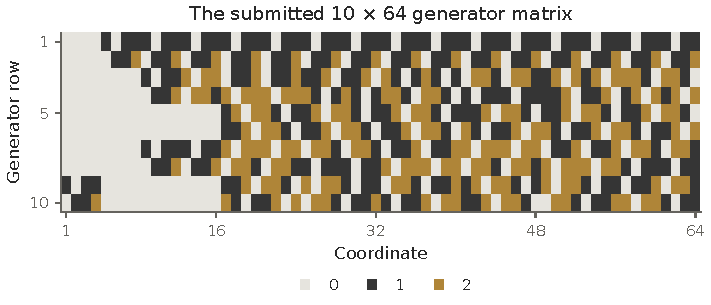
\includegraphics[width=\linewidth]{figs/appendix/case_trifference.pdf}\end{center}

\begin{constructionbox}[title=Construction and verification]
The answer is a $10\times64$ ternary generator matrix $G$. Its rows span a linear code
\[
C=\{uG:u\in\mathbb F_3^{10}\},\qquad \operatorname{rank}(G)=10,
\qquad |C|=3^{10}=59049.
\]
The coloured matrix above is the submitted generator: grey, black and gold denote 0, 1 and 2. The hyperplane test in Appendix~\ref{app:trifference_certificates} checks the separation condition without listing every triple of codewords. Both verifiers accepted the construction.
\end{constructionbox}

\begin{resultbox}[title=Measured quality]
\begin{tabularx}{\linewidth}{@{}XXX@{}}
Model construction & Construction baseline & Relative quality \\
\textbf{59,049 words} & 19,683 words & $59049/19683=\mathbf{3}$
\end{tabularx}
\end{resultbox}

A short certificate describes a code three times as large as the construction baseline, giving relative quality 3. The other three evaluated lengths test whether that quality extends further.

\appendixpage
\subsection{Schur colourings: successive advances on one scale}
\label{case:schur}
\textbf{Source:} published constructions. \textbf{Instance:} eight colours.

\begin{taskbox}[title=Task]
Colour $\{1,\ldots,N\}$ with eight colours so that no colour class contains a solution of $x+y=z$, including $x=y$. Larger $N$ gives a stronger construction.
\end{taskbox}

\begin{center}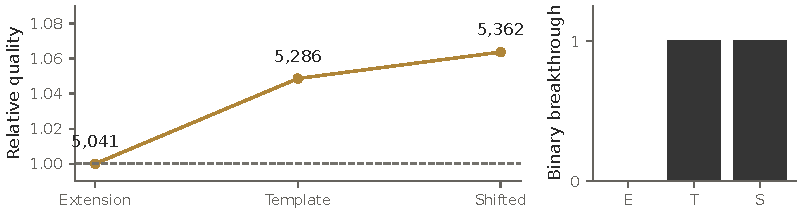
\includegraphics[width=\linewidth]{figs/appendix/case_schur.pdf}\end{center}

\begin{constructionbox}[title=Published constructions]
Recursive extension of the 1,680-element seven-colour construction reported by \citet{fredricksen2000schur} gives the historical reference
\[
N_0=3\cdot1680+1=5041.
\]
The template in \citet{rowley2021templates} gives $33\cdot160+6=5286$. Shifted templates give $10\cdot536+2=5362$~\citep{bengone2026schur}. We compare the published constructions against the same historical reference $N_0$.
\end{constructionbox}

\begin{resultbox}[title=Measured progress]
\centering\footnotesize\setlength{\tabcolsep}{5pt}
\begin{tabular}{@{}lrrr@{}}
\toprule
Published construction & $N$ & $N/5041$ & $\mathbf{1}\{N>5041\}$ \\
\midrule
Recursive extension~\citep{fredricksen2000schur} & 5,041 & 1.000 & 0 \\
Rowley template~\citep{rowley2021templates} & 5,286 & 1.049 & 1 \\
Shifted template~\citep{bengone2026schur} & 5,362 & 1.064 & 1 \\
\bottomrule
\end{tabular}

\captionof{table}{Selected published Schur constructions with eight colours, scored against the historical reference $N_0=5041$. The last column records whether the construction exceeds this reference. Citations identify the accounts used for each construction.}
\label{tab:history}
\end{resultbox}

Both advances count as one binary success, while relative quality preserves their different magnitudes. The current benchmark uses 5,362 as the eight-colour reference and extends the challenge by increasing the number of colours under the same construction rule.
